%\documentclass[11pt,twocolumn]{article}
\documentclass{llncs}

\usepackage{graphicx}
\usepackage{url}
\usepackage{hyperref}
\usepackage{subcaption}         % include subfigure
\bibliographystyle{splncs03}

\begin{document}

\title{Early evaluation of the hybrid cluster with torus interconnect aimed at cost-effective molecular-dynamics simulations}

\author{%
Vladimir~V.~Stegailov\inst{1},
Alexander~Agarkov\inst{2},
Sergey~Biryukov\inst{2},
Timur~Ismagilov\inst{2},
Nikolai~Kondratyuk\inst{1}\inst{3},
Evgeny~Kushtanov\inst{2},
Dmitry~Makagon\inst{2},
Anatoly~Mukosey\inst{2},
Alexander~Semenov\inst{2},
Alexey~Simonov\inst{2},
Vyacheslav~Vecher\inst{1}\inst{3}
}
%
\authorrunning{V.~Stegailov et al.} % abbreviated author list (for running head)
%
\institute{Joint Institute for High Temperatures of RAS, Moscow, Russia\\
\and NICEVT, Moscow, Russia\\
\and Moscow Institute of Physics and Technology, Dolgoprudny, Russia\
%FIXME Владимир, может быть, не очень хорошо здесь указывать почту из ВШЭ?
\email{v.stegailov@hse.ru}
}

\maketitle

\begin{abstract}
In this paper, we describe the Desmos cluster that consists of 32 hybrid nodes connected by a low-latency high-bandwidth torus interconnect. The interconnect is based on the Angara NIC that supports 3D and 4D torus network topology. We describe the corresponding ASIC structure and the software stack (shmem and MPI including). Firstly, this cluster is aimed at cost-effective classical molecular dynamics calculations. We present strong and weak scaling benchmarks for GROMACS and LAMMPS. Secondly, the cluster serves as a test bed for the Angara interconnect and verifies its ability to unite large MPP systems and to speed-up effectively MPI-based applications.
\end{abstract}


\section{Introduction}


\section{Related work}

\subsection{Scalability of classical MD on supercomputers}


\section{Cluster ``Desmos''}

\begin{table}[h]
\caption{\label{tab:systems}Desmos cluster system configuration.}
\begin{center}
\renewcommand{\arraystretch}{1}
\begin{tabular}{|p{33mm}|p{80mm}|}
\hline
\textbf{Server} & Supermicro SuperServer 1018GR-T\\
\hline
\textbf{Processor} & Xeon E5-1650 v3 (6 cores, 3.0 GHz)\\
\hline
\textbf{GPU} & Nvidia GeForce GTX 1070 (1920C, 8 GB GDDR5)\\
\hline
\textbf{Memory} & DDR4 8 GB\\
\hline
\textbf{Number of nodes} & 32\\
\hline
\textbf{Interconnect} & Angara 4D-torus $4\times2\times2\times2$\\
\hline
\textbf{Operating system} & SLES 11 SP4 \\
\hline
\textbf{Compiler} & Intel Parallel Studio XE 2017 \\
\hline
\textbf{MPI} & Angara MPI (based on MPICH 3.0.4)\\
\hline
\end{tabular}
\end{center}
\end{table}

\subsection{GPU Testing}
The Nvidia GTX 1070 cards have no memory errors correction
(ECC) in contrast to the professional accelerators. For this reason
it was necessary to make sure that there is no hardware memory errors in each GPU.


Testing of each GPU was performed using MemtestG80 \cite{Haque:2010:HDS:1844765.1845231}.
Testing was performed on the available memory of the accelerator (8 GB) and wasted at least
4 hours (depending on the number of test iterations). Testing time was chosen on the basis of the results obtained in the paper \cite{Kutzner2015BestBF} and restrictions 
imposed by the number of cards and the total time of the test the entire batch. There are no errors detected during the testing process.

\subsection{Angara Interconnect}
%FIXME to dmvkt: BG, Cray, Tofu, Extoll

Angara interconnect is a Russian-designed communication network with torus topology. Inteconnect chip was developed by JSC NICEVT and manufactured by TSMC with 65 nm process. The chip supports deadlock-free adaptive routing based on bubble flow control \cite{Puente:1999:ABR:850940.852882},  direction ordered routing \cite{Adiga:2005:BGT:1665957.1665963}, \cite{Scott96thecray} and initial and final hops \cite{Scott96thecray} for fault tolerance.

Each node has a dedicated memory region available for remote access (read, write, atomic operations) from other nodes to support the OpenSHMEM and PGAS languages. Multiple parallel programming models are supported, including MPI, OpenMP, OpenSHMEM.

The network adapter is a PCI Express extension card that is connected to the adjacent nodes by up to 6 cables (or up to 8 with an extension card). The following topologies are supported: ring, 2D, 3D and 4D torus (or grid). 


\begin{figure}
\centering
  %\includegraphics[width=0.8\textwidth]{fig.pdf}
\caption{The scheme of the ``Angara'' chip.}
\end{figure}


%\subsection{Software stack (MPI)}

%Including analytic estimates that show no need for extra MPI tuning below 256 nodes




Description

Early HPL performance

Energy consumption

\begin{figure}[h]
\centering
  %\includegraphics[width=0.8\textwidth]{fig.pdf}
\caption{The photo of one ``Desmos'' node and the photo of the rear side of the rack with cabling.}
\end{figure}

%\begin{figure}[h]
%\centering
%  %\includegraphics[width=0.8\textwidth]{fig.pdf}
%\caption{The scheme of the links between 32 cluster nodes (4x2x2x2).}
%\end{figure}


\section{Experimental Results}

\begin{figure}[h!]
\centering
   \begin{subfigure}{0.48\textwidth}
  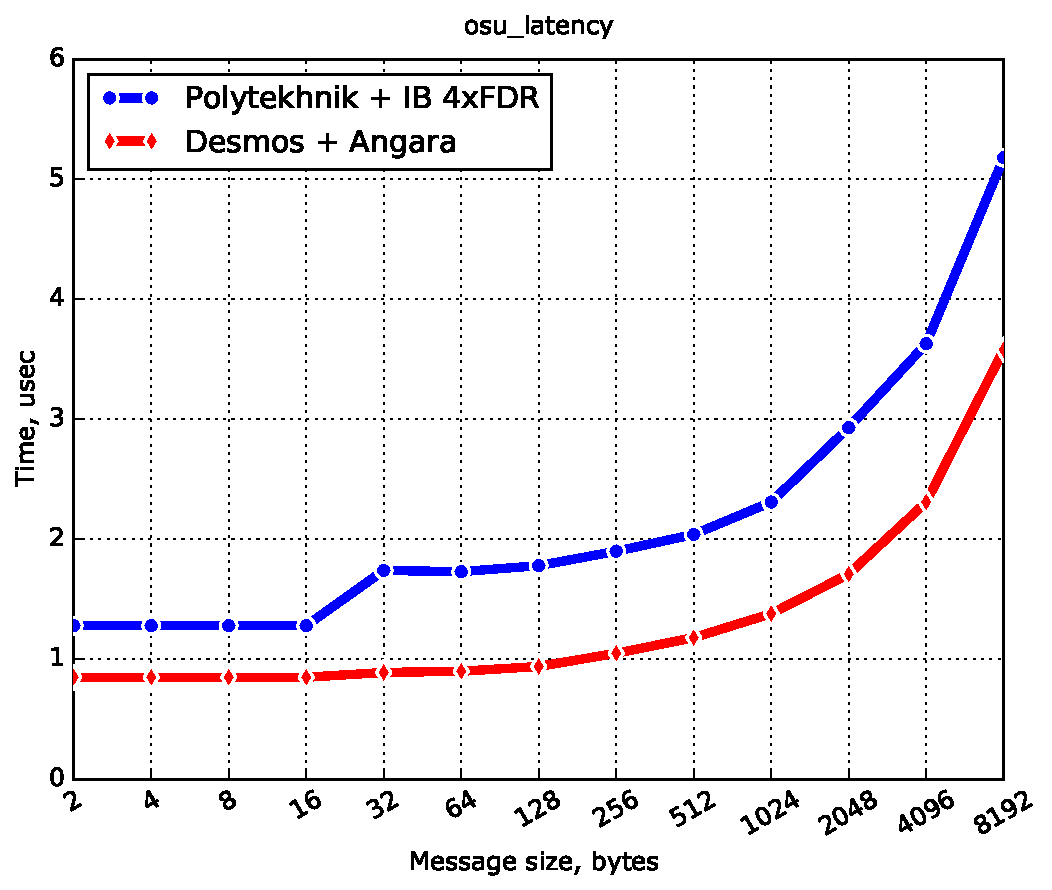
\includegraphics[width=1\textwidth]{img/osu_latency.pdf}\caption{}
  \end{subfigure}
  \begin{subfigure}{0.48\textwidth}
  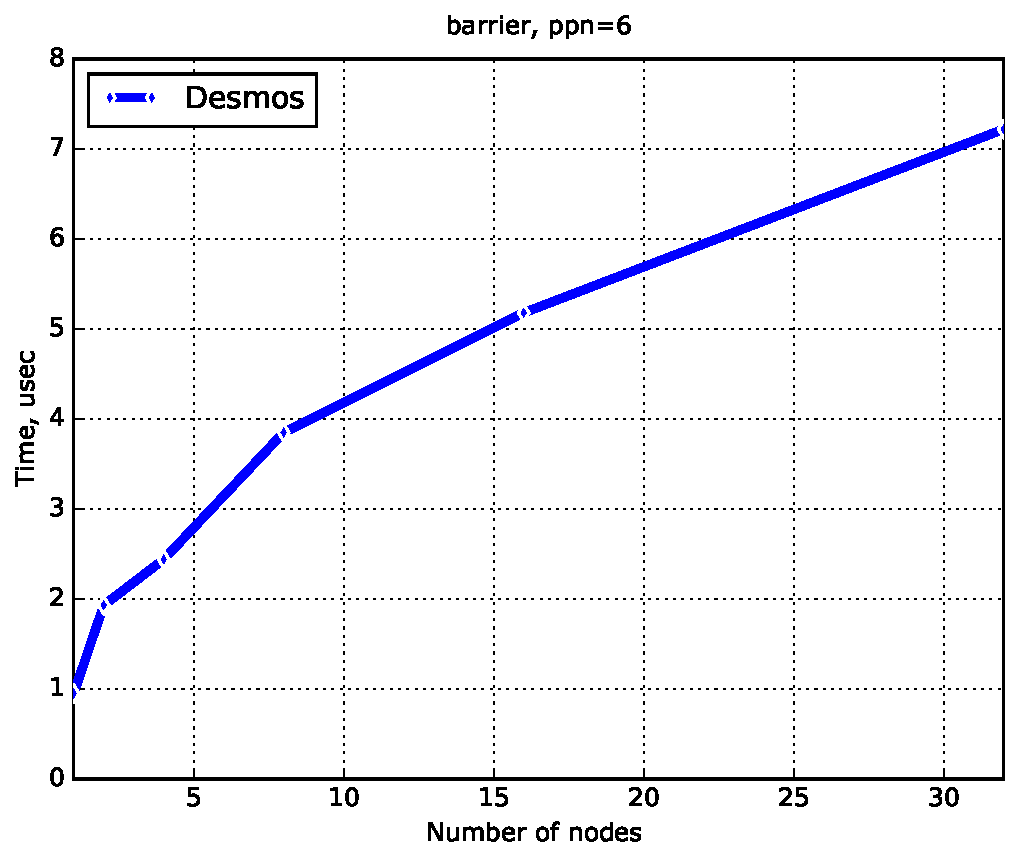
\includegraphics[width=1\textwidth]{img/barrier_ppn=6.pdf}\caption{}
   \end{subfigure}
\caption{(a) Communication latency between two adjacent Desmos nodes (OSU Micro-Benchmarks 5.3.2). (b) Intel MPI Benchmarks 2017 MPI\_Barrier, processes per node (ppn) = 6.}
\end{figure}

\begin{figure}[h!]
\centering
   \begin{subfigure}{0.48\textwidth}
  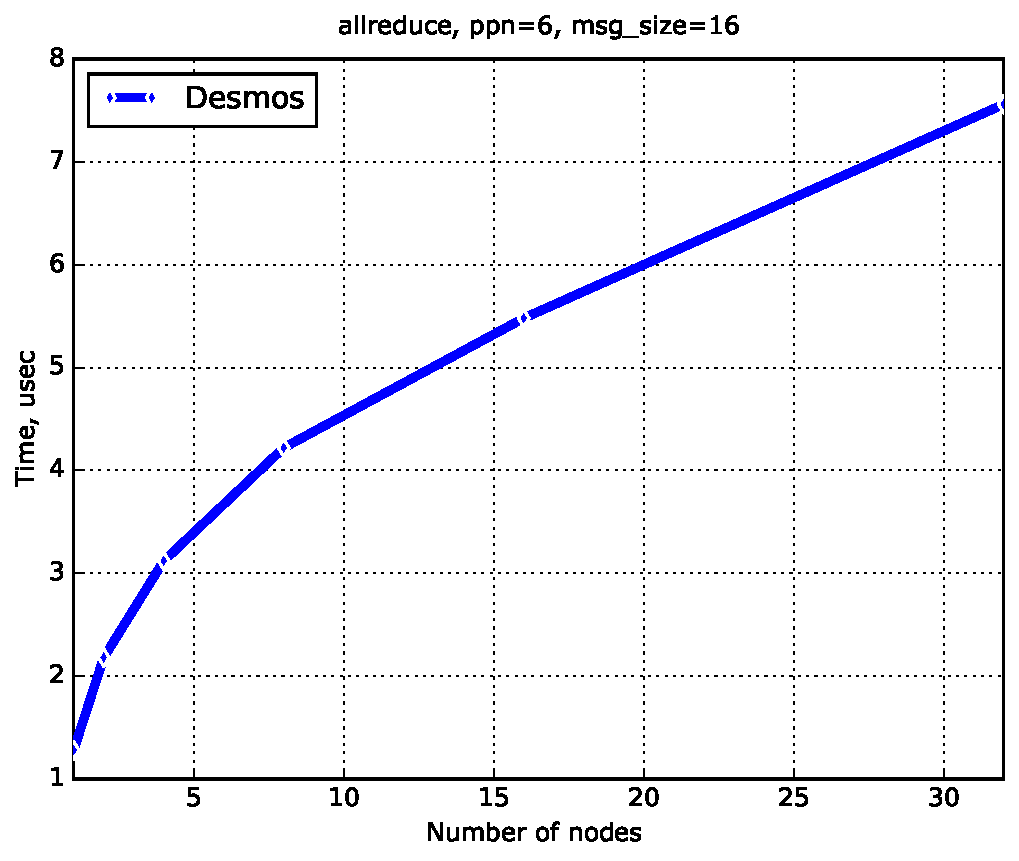
\includegraphics[width=1\textwidth]{img/allreduce_ppn=6_size=16.pdf}\caption{}
  \end{subfigure}
  \begin{subfigure}{0.48\textwidth}
  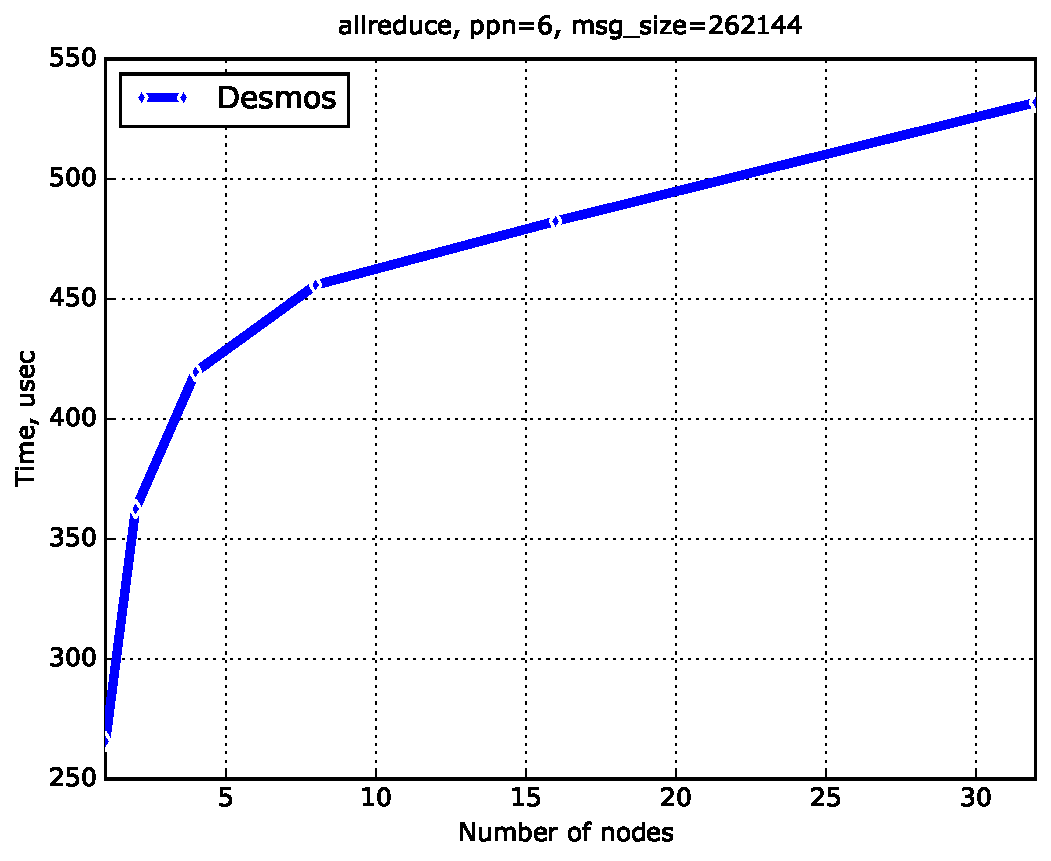
\includegraphics[width=1\textwidth]{img/allreduce_ppn=6_size=262144.pdf}\caption{}
   \end{subfigure}
\caption{FIXME: REMOVE?? Intel MPI Benchmarks 2017 MPI\_Allreduce, ppn = 6 (a) message size = 16 bytes (b) message size = 256 KB. }
\end{figure}

\subsection{MD Benchmarks}

ApoA1 model (100000 atoms) with GROMACS – comparison with BlueGene, Cray and other large machines.

Large LJ system with LAMMPS on 32 nodes – influence on special decomposition mapping on torus topology.

Comparison ns/day vs hardware cost.

\begin{figure}[h]
\centering
  %\includegraphics[width=0.8\textwidth]{fig.pdf}
\caption{ApoA1 benchmark. Timestep per 1 atom per 1 MD step vs $R_{peak}$. The comparison of different systems.}
\end{figure}

\begin{figure}[h]
\centering
  %\includegraphics[width=0.8\textwidth]{fig.pdf}
\caption{Time vs cost. Comparison with the published results for GROMACS.}
\end{figure}


\section{Conclusions}

The work of the JIHT team (N.K., V.S. and V.V.) was supported by the grant No.\,14-50-00124 of the Russian Science Foundation (this work includes the development of the cluster node architecture, the preliminary benchmarks, the purchase of the ``Desmos'' cluster). The NICEVT team developed the ``Angara'' interconnect and the corresponding low-level software stack, built and tuned the ``Desmos'' cluster).


\bibliography{references}

\end{document}
